\graphicspath{{./figures}}

\section{Ground Station PCB}

The ground station PCB was manufactured in-house. A figure of the PCB with components assembled, as well as a helical antenna attached for initial development, and a simple monopole GPS antenna, is shown in Figure \ref{fig:groundStationPCB}. Due to a few incorrect layouts on the PCB, some additional wired connections were made. A list of errata can be found in Appendix \ref{sec:appendix_pcb_errata}.


\begin{figure}[!htb]
  \begin{minipage}{.49\textwidth}
    \centering
    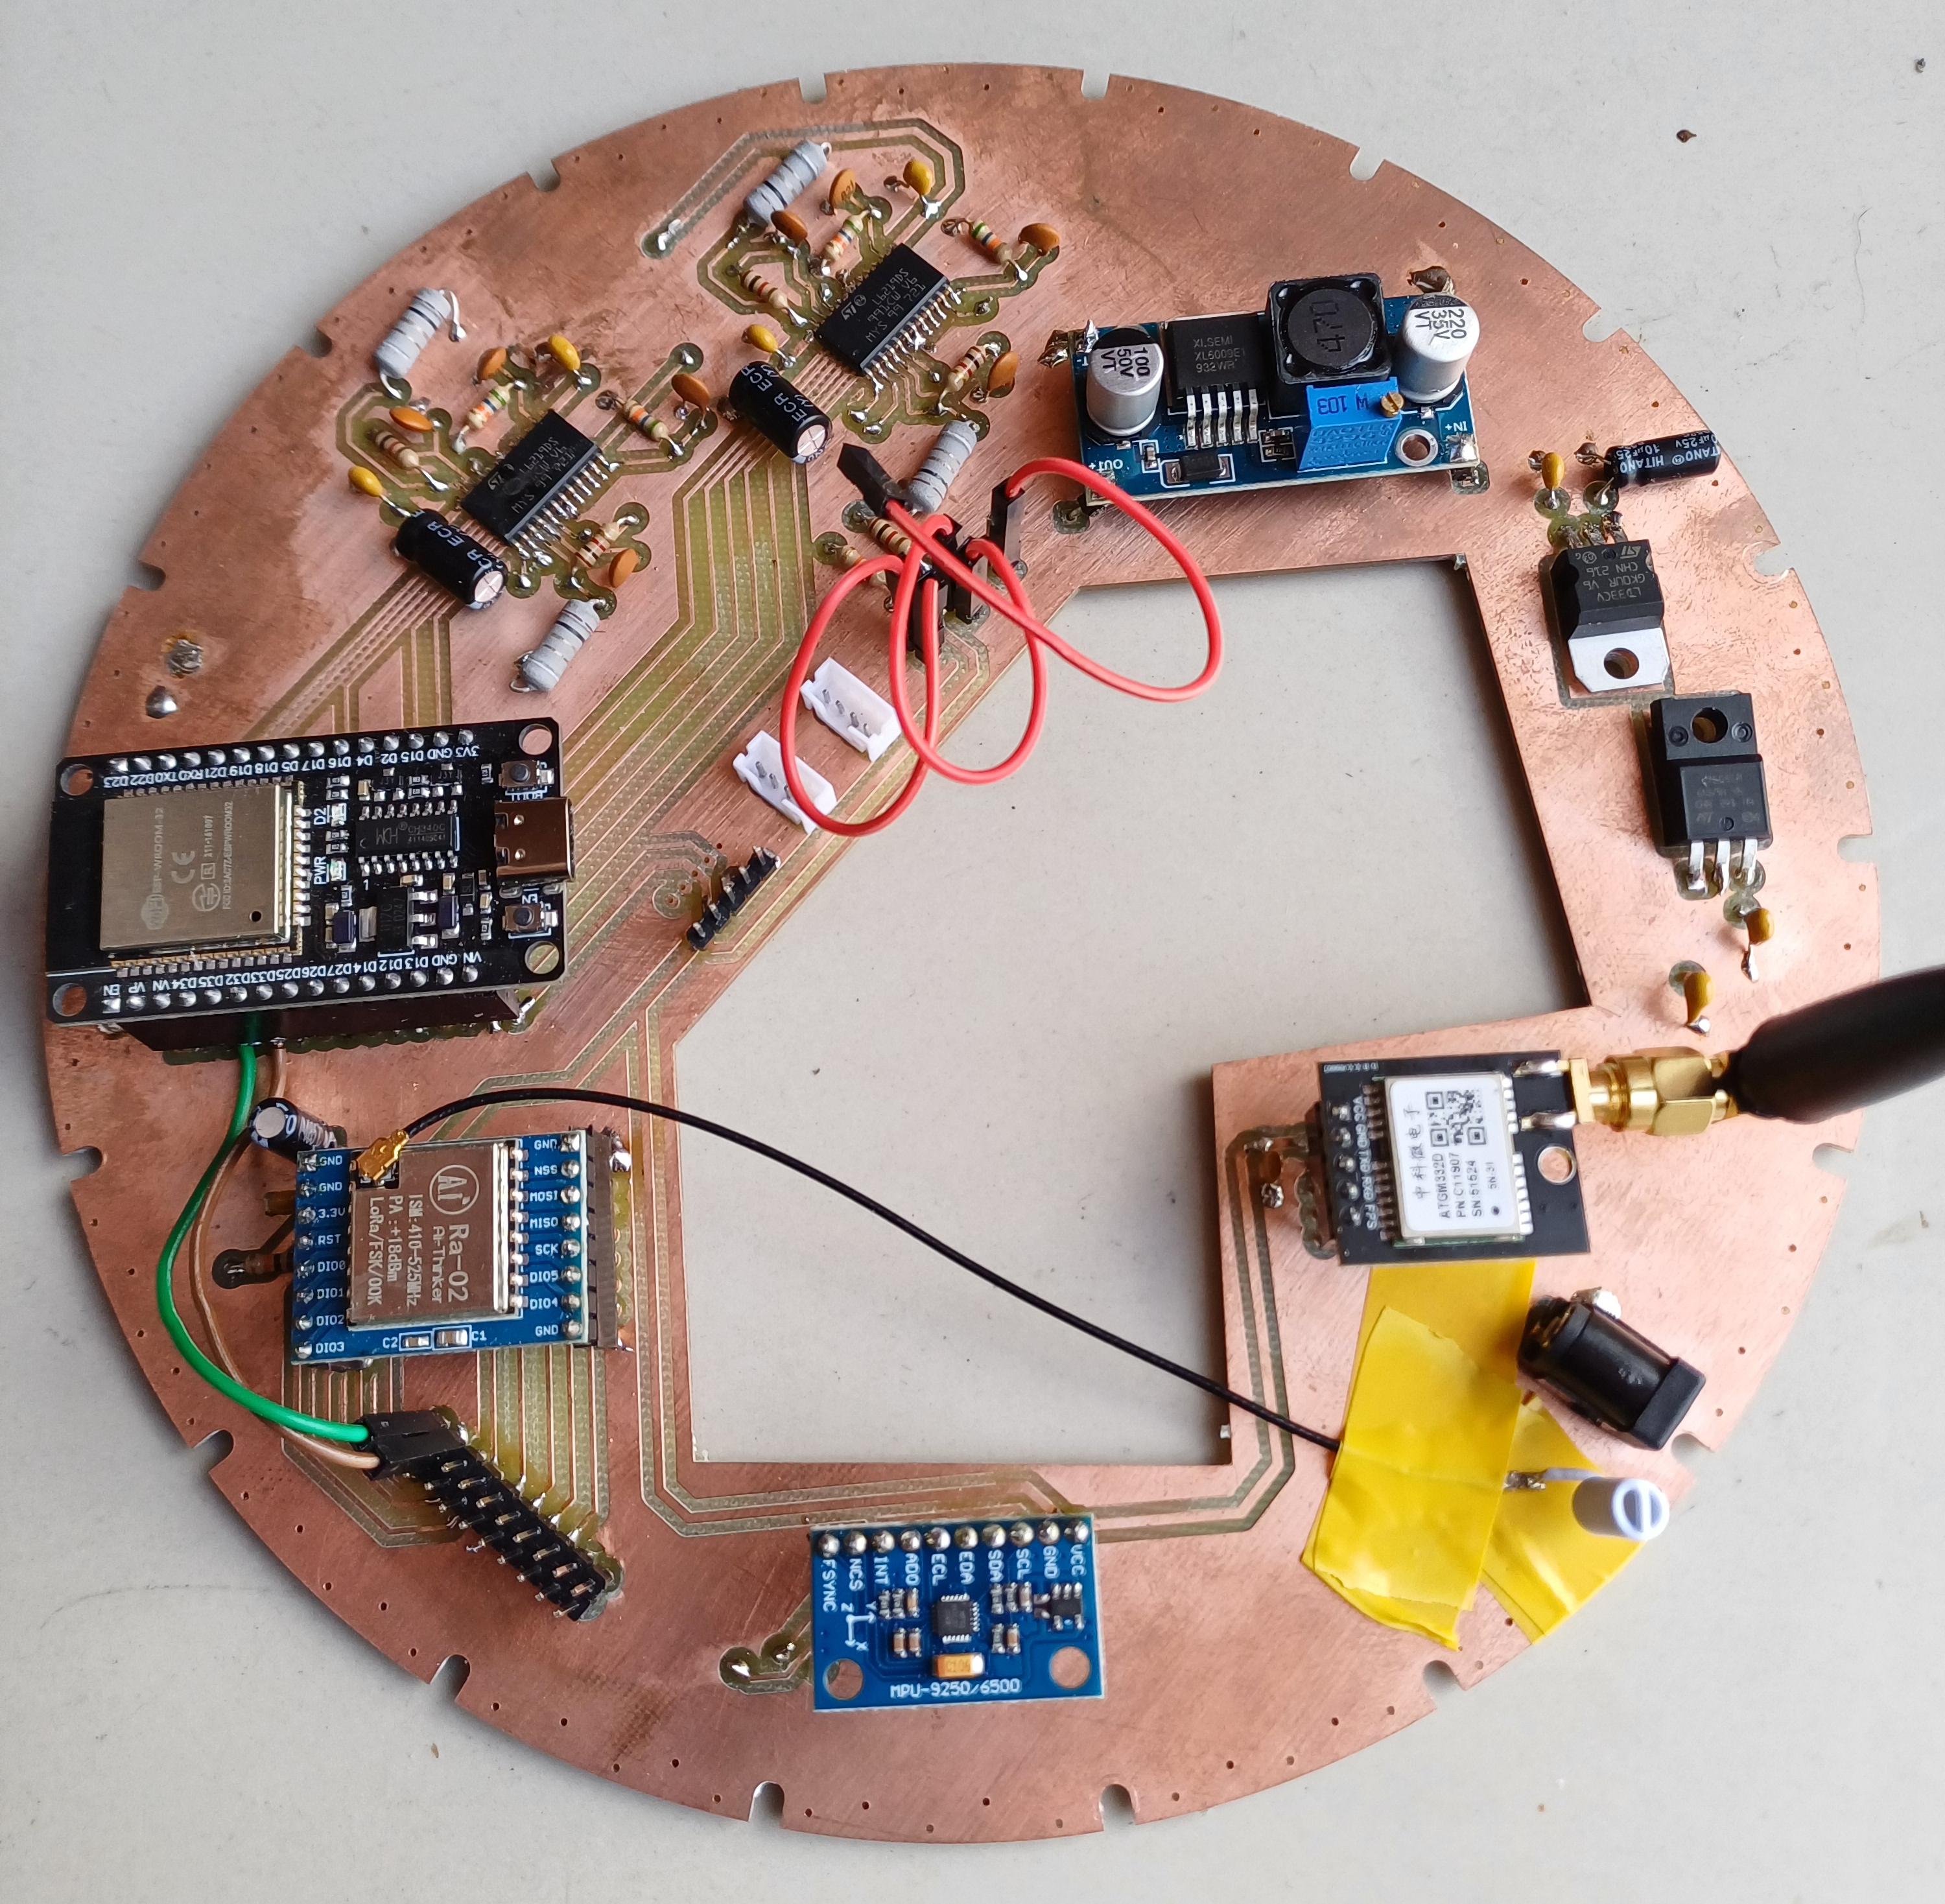
\includegraphics[width=0.8\linewidth]{groundStationPCB}
    \caption{Ground Station PCB Implementation}
    \label{fig:groundStationPCB}
  \end{minipage}
  \begin{minipage}{.49\textwidth}
    \centering
    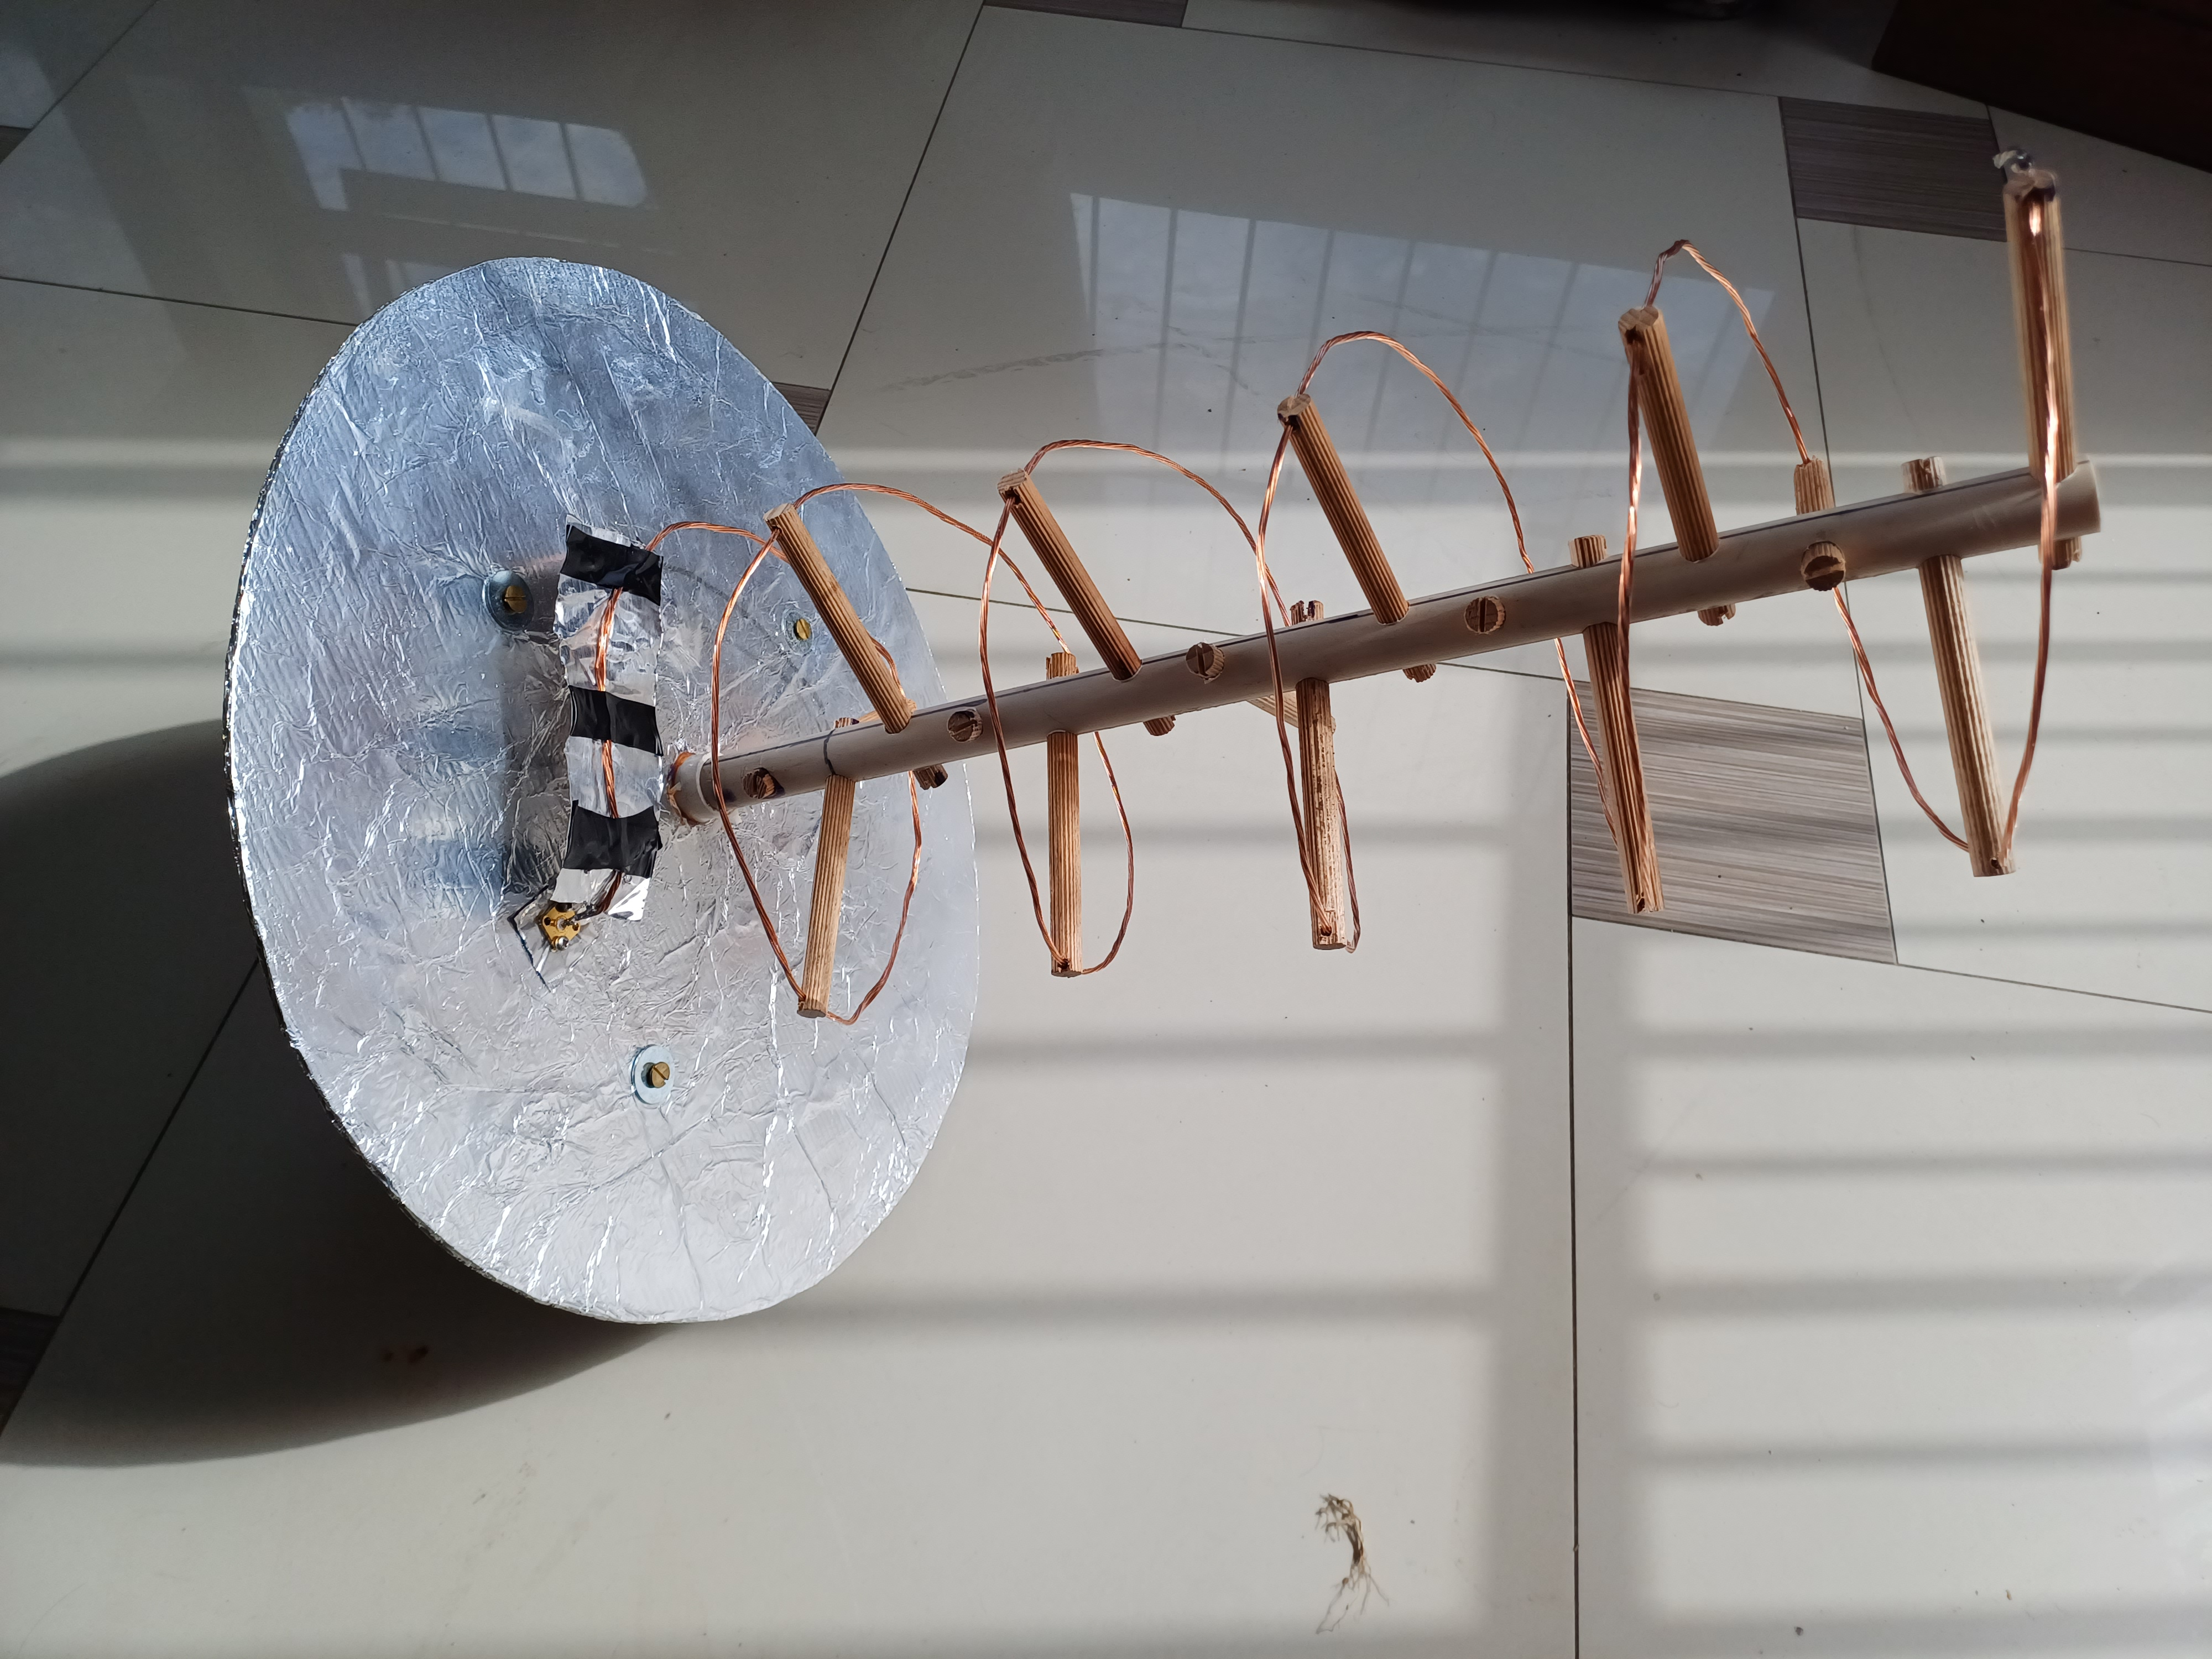
\includegraphics[width=0.95\linewidth]{gsAntennaOriginal}
    \caption{Ground Station Initial Antenna Implementation}
    \label{fig:gsAntennaOriginal}
  \end{minipage}
\end{figure}